\documentclass{nature}
\bibliographystyle{naturemag}

\usepackage{amssymb}
\usepackage{graphicx}
\graphicspath{{figures/}}
%\usepackage{lineno}
%\linenumbers

% #magic #hack to make figures appear
\makeatletter
\let\saved@includegraphics\includegraphics
\AtBeginDocument{\let\includegraphics\saved@includegraphics}
\renewenvironment*{figure}{\@float{figure}}{\end@float}
\makeatother


% TODO:
% [ ] Re-make number of pre-prints posted per sub-field of q-bio into one panel.
% [ ] Re-make number of pre-prints in q-bio by author as linear.
% [ ] Nice-ify all figures.
% [ ] Poisson process model predictions for all primary research fields.


\usepackage{color}

\usepackage[dvipsnames]{xcolor}

\definecolor{mygray}{gray}{0.6}


\newcommand{\todo}[1]{\textcolor{gray}{#1}}
\newcommand{\arxiv}{arXiv}

% I don't suggest this title; this is a placeholder.
\title{What pandemic?}


\author{Andrew R. Casey$^{\ast,1,2,}$,
        Ilya Mandel$^{\ast,1,2}$,
        Prashun?, 
        and friends?
}

\begin{document}

\maketitle

\begin{affiliations}
	\item School of Physics \& Astronomy, Monash University, Clayton 3800, Victoria, Australia
	\item Center of Excellence for Astrophysics in Three Dimensions (ASTRO-3D), Australia
\end{affiliations}

\begin{abstract}
	% Context.
	`\emph{Publish or perish}' is an expression that refers to the pressure placed on academics to consistently publish research to ensure a successful career in academia.
	% Define the gap, or question.
	With a global pandemic that has changed how businesses operate, has it also changed the academic publishing system?
	% Here we show.
	Here we show that academics are collectively posting just as many publications as if there were no pandemic. 
	This remains true across nearly all fields of research, including those focussed on theoretical and experimental research.
	The most significant change in academic publishing is seen in biology, where there was a doubling of pre-prints posted in 2020. 
	However, most of these extra pre-prints are not written by, or with, biologists.
	\todo{At least half} of the excess biology pre-prints are entirely authored by researchers from other fields, primarily physicists.
	No broad impact is found between theoretical and experimental research.
	Reduced access to experimental laboratories seems to have motivated researchers to publish more papers (overall) based on work that was already in preparation. The full impact of the pandemic on academic publishing may not yet be fully realised.	
\end{abstract}


Peer-reviewed publications are the primary measure of productivity in academia. The \arxiv\ is a distribution service for research publications before they are printed in a journal (i.e., a pre-print). A pre-print on the \arxiv\ does not ensure that the contents have already passed peer-review, but most material on the \arxiv\ eventually goes through peer-review because it is now standard in many research fields to post pre-prints to the \arxiv\ either during or after the peer-review process. For this reason, the number of pre-prints posted to the \arxiv\ reflects the number of peer-reviewed publications written at any time.


We retrieved metadata for 1.38 million pre-prints posted on the \arxiv\ between April 2007 and December 2020. The metadata includes the creation date, research field(s), title, author name(s), abstract, and other miscellaneous information. These data show that there is an increasing number of publications each year in nearly every field  (Figure~\ref{fig:pre-prints-segmented-by-field}). These long-term trends are relatively predictable from year to year, allowing us to measure any change in academic productivity due to the current pandemic.


In most fields there was no impact on pre-print rates due to the COVID-19 pandemic. We used the number of publications from January 2008 to January 2020 to predict the expected number of publications in 2020 in a given field (see Methods). The listed number of publications in 2020 agree excellently with the model predictions in most fields. The most significant deviation is in quantitative biology (\arxiv\ code `q-bio'), where 2020 saw about double the number of pre-prints than expected (\todo{$X^{X}_{X}$} expected, \todo{$Y$} observed). The increase in quantitative biology is dominated by  pre-prints in the sub-field of \emph{Populations and Evolution} (q-bio.PE; Figure~\ref{fig:q-bio-pre-prints-with-entirely-new-authors}), and the most frequent abstract terms relate to the SARS-COV-2 disease, the COVID-19 virus, or the associated pandemic.


An increase in biology research during a global pandemic is not surprising. However, the data suggests that at \todo{least half} of these additional biology pre-prints were not written by established biologists. The number of new authors appearing in any field is representative of how quickly a field is growing. The number of new authors in quantitative biology peaked in 2020 (Figure~\ref{fig:new-authors-segmented-by-field}), while the number of new authors in all other fields remained steady. The sudden influx of new authors cannot be explained by large newly-formed collaborations working together to tackle the impending pandemic (Figure~\ref{fig:q-bio-pre-prints-segmented-by-author-count}). 


The increase in pre-prints (and new authors) is driven by small (1-4) groups of authors who had never before posted pre-prints to quantitative biology before, either as leading- or co-author  (Figure~\ref{fig:pre-prints-with-entirely-new-authors}). It is possible that the COVID-19 pandemic inspired hundreds of established biologists, who had never posted pre-prints to the \arxiv\ before, to quickly use these services disseminate their research. This can only explain some of the excess biology pre-prints in 2020. 
We examined the number of pre-prints posted in \emph{Populations and Evolution} (q-bio.PE) where those author names had never appeared in any quantitative biology (q-bio) field before, but those names do appear in other \arxiv\ fields (Figure~\ref{fig:q-bio-pre-prints-with-author-overlap}). This gives a measure of the number of common names between different fields before the pandemic, which is about 1-3\%. In 2020 most of the pre-prints in \emph{Populations and Evolution} that are \emph{entirely} written by `new' authors (non-biologists) are author names from other fields, primarily physicists and mathematicians. The fields with the largest number of unique names are, in order: computer science, physics, condensed matter, math, and astrophysics. While it is more likely to have names overlapping between biology and computer science (the largest field by unique names) by chance, the newly authored pre-prints in quantitative biology in 2020 are driven by physicists and mathematicians. 
Taking the number of pre-prints in \emph{Populations and Evolution} (q-bio.PE) where no author has appeared before in that sub-field, at least 40\% of these pre-prints are written by researchers from other fields. A careful cross-match of biology pre-prints with Google Scholar profiles shows that this statement is not conflated by two researchers with the same name that work in different fields. While some biologists continued to post to \arxiv\ for the first time in 2020, the sharp increase in biology pre-prints in 2020 is driven by researchers from other fields.


This could be viewed as a good or bad thing, depending on your view. Is it still considered multi-disciplinary research -- a research trait fertilised by many institutions worldwide -- to publish in another field without any subject domain experts? Are academics spending time trying to advance efforts against the most significant problem to face society this year, or are some jumping on a citation-laden bandwagon? The impact of these pre-prints is hard to measure. The number of citations are routinely used as a measure of research impact, but that metric becomes less useful in a period where pre-prints are being written (and cross-citing each other) faster than those pre-prints are being read.



While the number of pre-prints within primary research fields has remained largely unchanged during the pandemic, there have been noticeable changes within specific sub-fields. Border restrictions have obviously limited field work and the capacity to attend conferences. In the field of high energy physics (lattice), pre-prints tend to peak around December each year as research presented at the International Symposium on Lattice Field Theory conference is posted on \arxiv. In 2020 no Lattice Field Theory conference was held\footnote{The last Lattice Field Theory conference was coincidentally held in Wuhan, Hubei, China.}, so no accompanying pre-prints were posted (Figure~\ref{fig:new-authors-segmented-by-field}). 

Even limiting access to compute facilities may have had a substantial effect on theoretical research. Within the field of computational physics (physics.comp-ph) the first half of 2020 saw a slight increase in pre-prints that was consistent with the rise in recent years. By June 2020 that peak began to fall, and continued to do so until the extent of the data (January 2021), where new pre-prints were at the lowest level seen in about five years. If this drop is a causal effect of the pandemic, it is the strongest relative decline seen in any sub-field.


Experimental laboratories have been forced to close, or remain open with reduced time and capacity. Access to laboratories is critical for condensed matter research, so it is reasonable to expect a sharp decline in pre-prints, but the exact opposite is observed: there were 20\% more pre-prints posted on material science (cond-mat.mtrl-sci) than in previous years (Figure~\ref{fig:winners-and-losers-of-covid}). Materials science is a sub-field of condensed matter focusses on laboratory methods and techniques. Usually these techniques are developed as part of an ongoing experiment, and then published separately once the primary (`more interesting') research is complete. Without access to laboratories, this increase may be a consequence of `writing up what we can': a motivation to publish existing work that would otherwise be neglected due to ongoing laboratory work. However, there were no accompanying sharp declines in any other categories of materials science: overall there were more publications across all fields of condensed matter, not fewer. Many research projects take months or years to complete. It is reasonable to suspect that the full effect of the pandemic has yet to be realised on pre-print counts, while academics publish what they can within ongoing restrictions.

\noindent\todo{physics.soc-ph saw a bump due to COVID-related research}


 \begin{figure}
     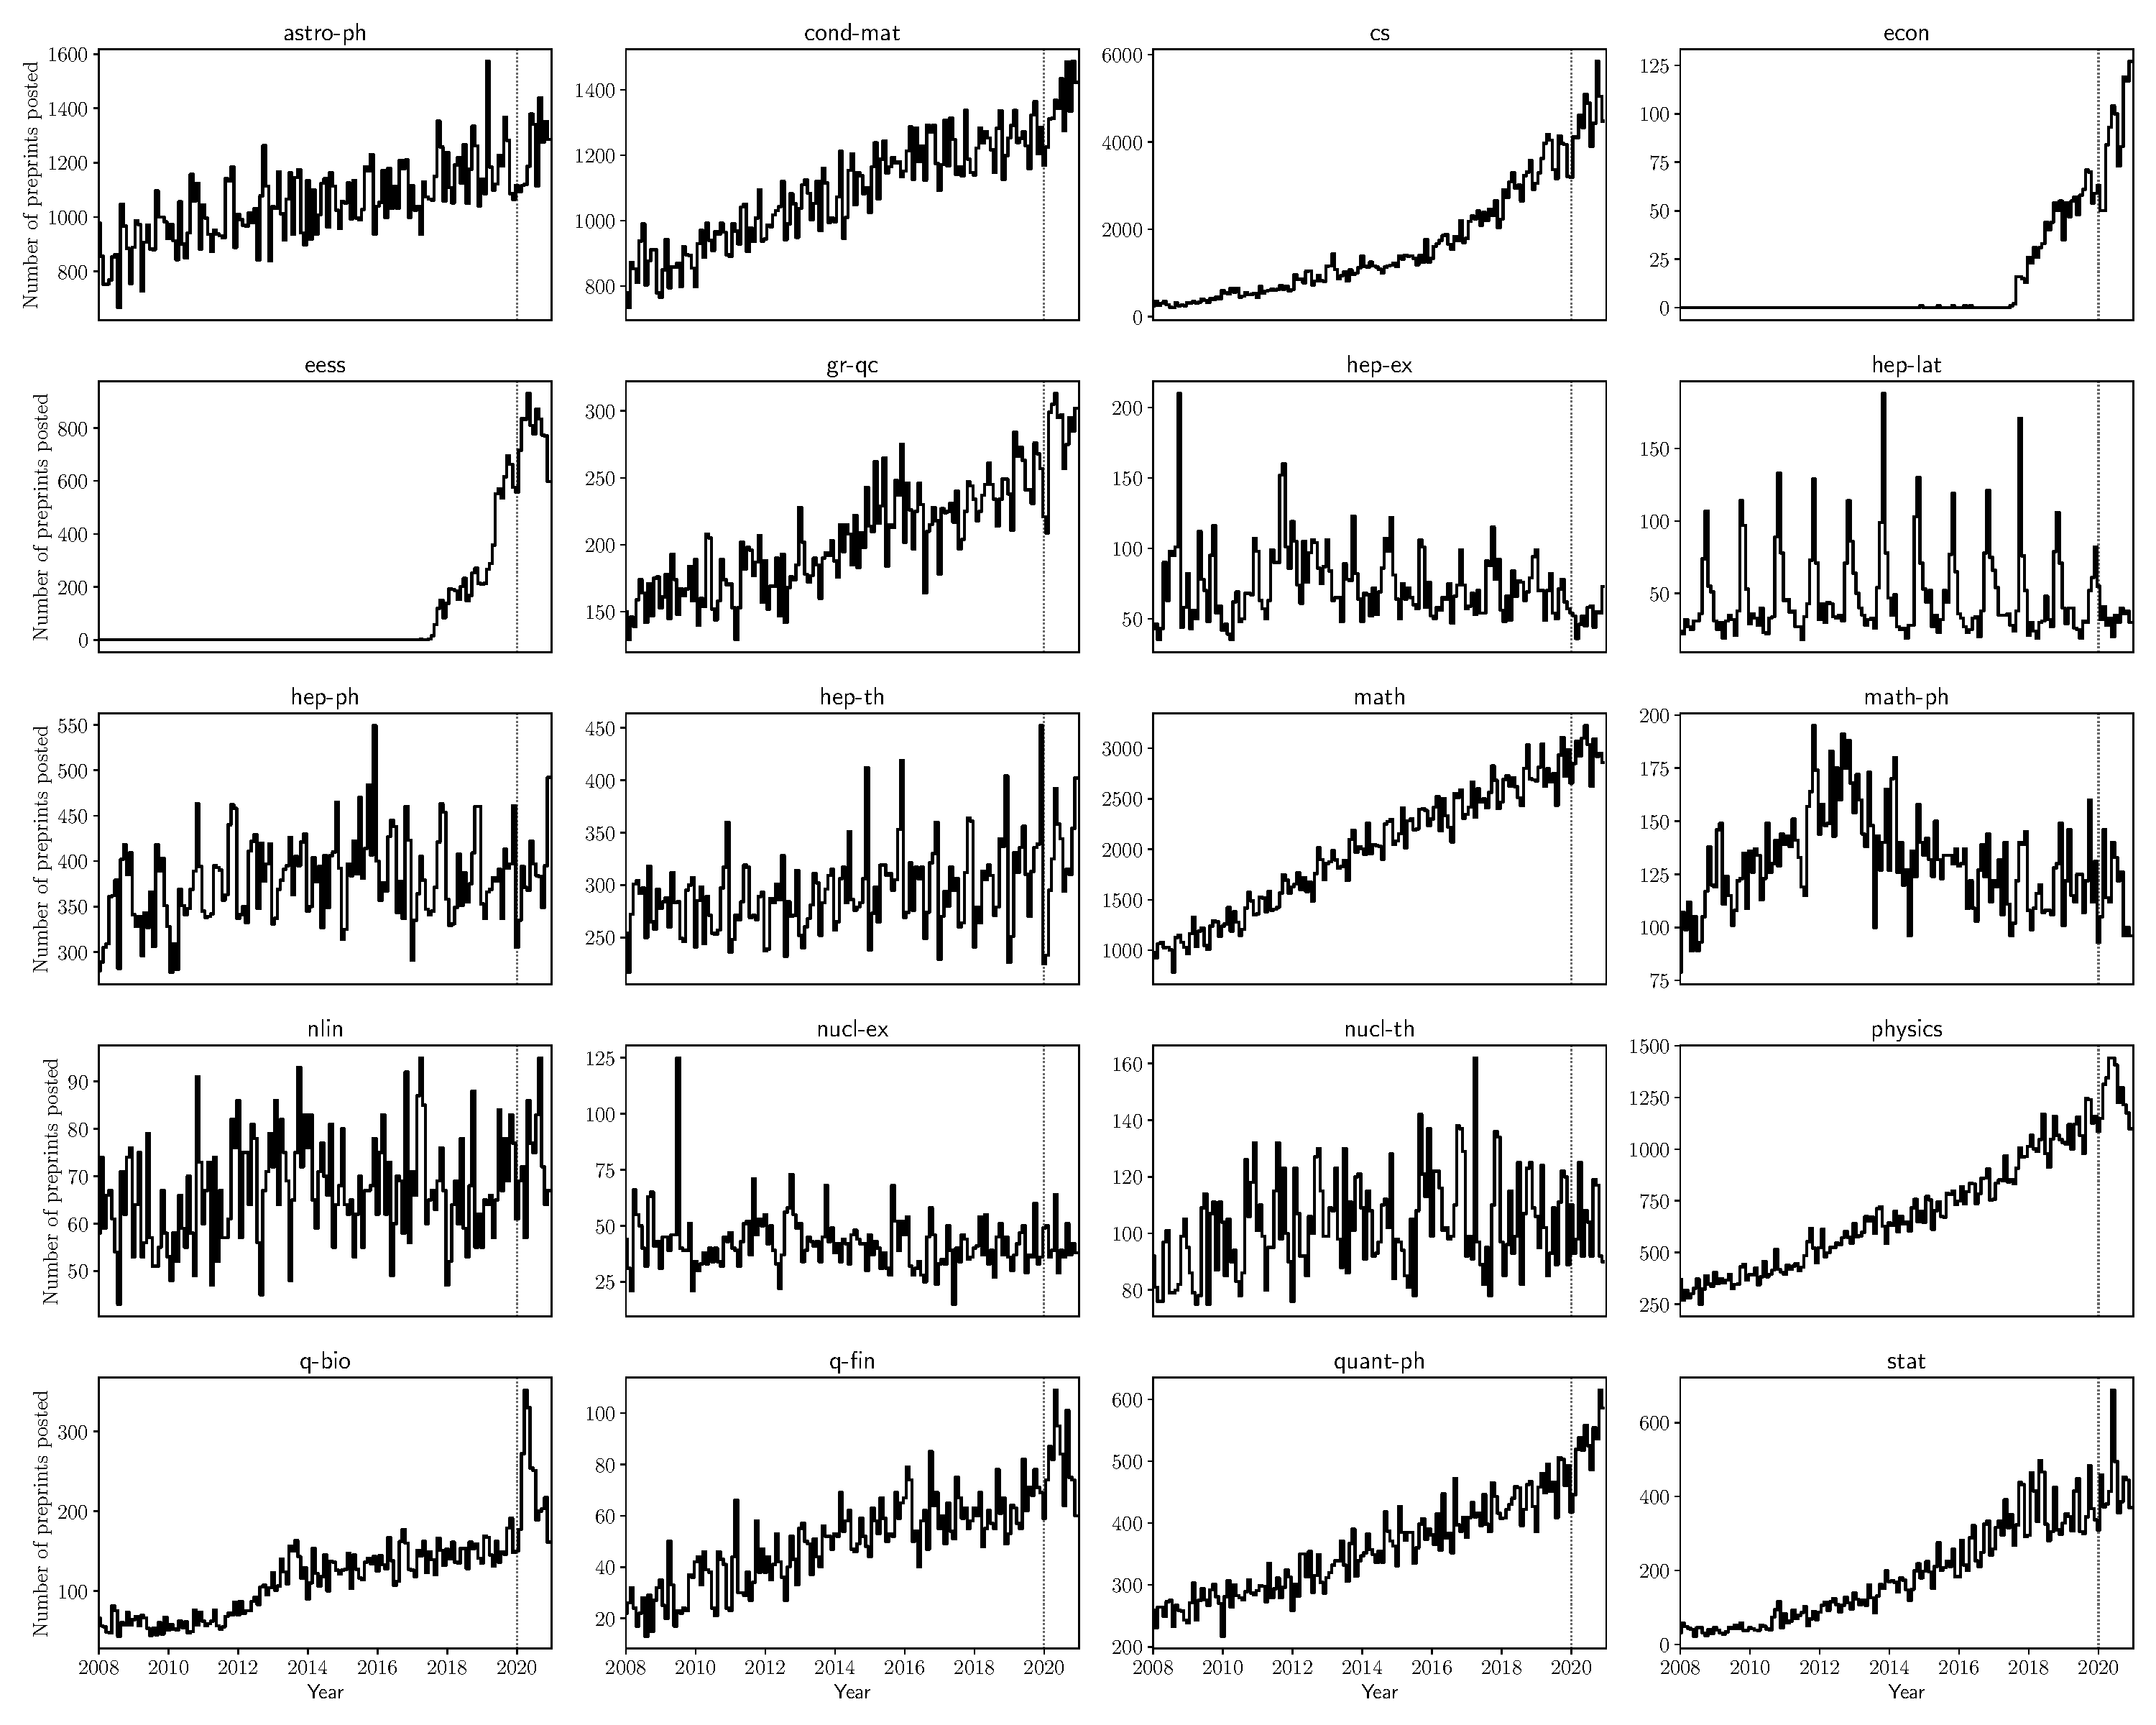
\includegraphics[width=\textwidth]{pre-prints-segmented-by-field}
     \caption{Most fields saw no change in the number of pre-prints posted due to the COVID-19 pandemic. The number of pre-prints continued to increase each year in most fields. \todo{The model.} The exception is quantitative biology (q-bio), where the spike in 2020 is in part caused by COVID-19 related pre-prints authored by people who are non-established biologists.}
     \label{fig:pre-prints-segmented-by-field}
 \end{figure}
 
\begin{figure}
	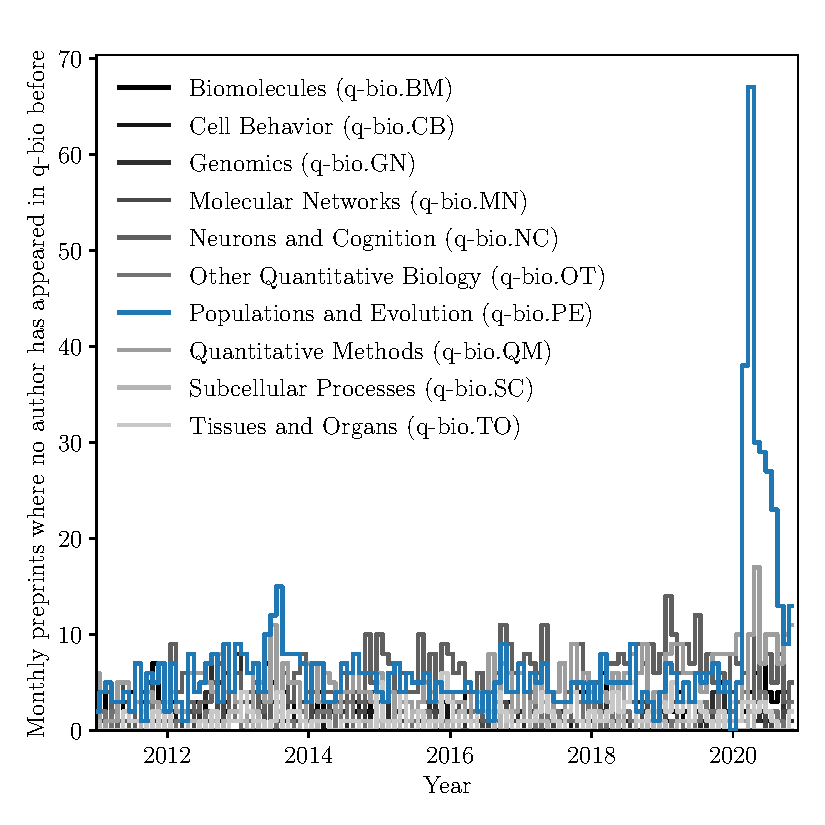
\includegraphics[width=\textwidth]{q-bio-pre-prints-with-entirely-new-authors}
	\caption{The number of pre-prints posted in sub-fields of quantitative biology where all authors have never before appeared in the biology literature. \todo{Re-make to single panel.}}
	\label{fig:q-bio-pre-prints-with-entirely-new-authors}
\end{figure}

\begin{figure}
	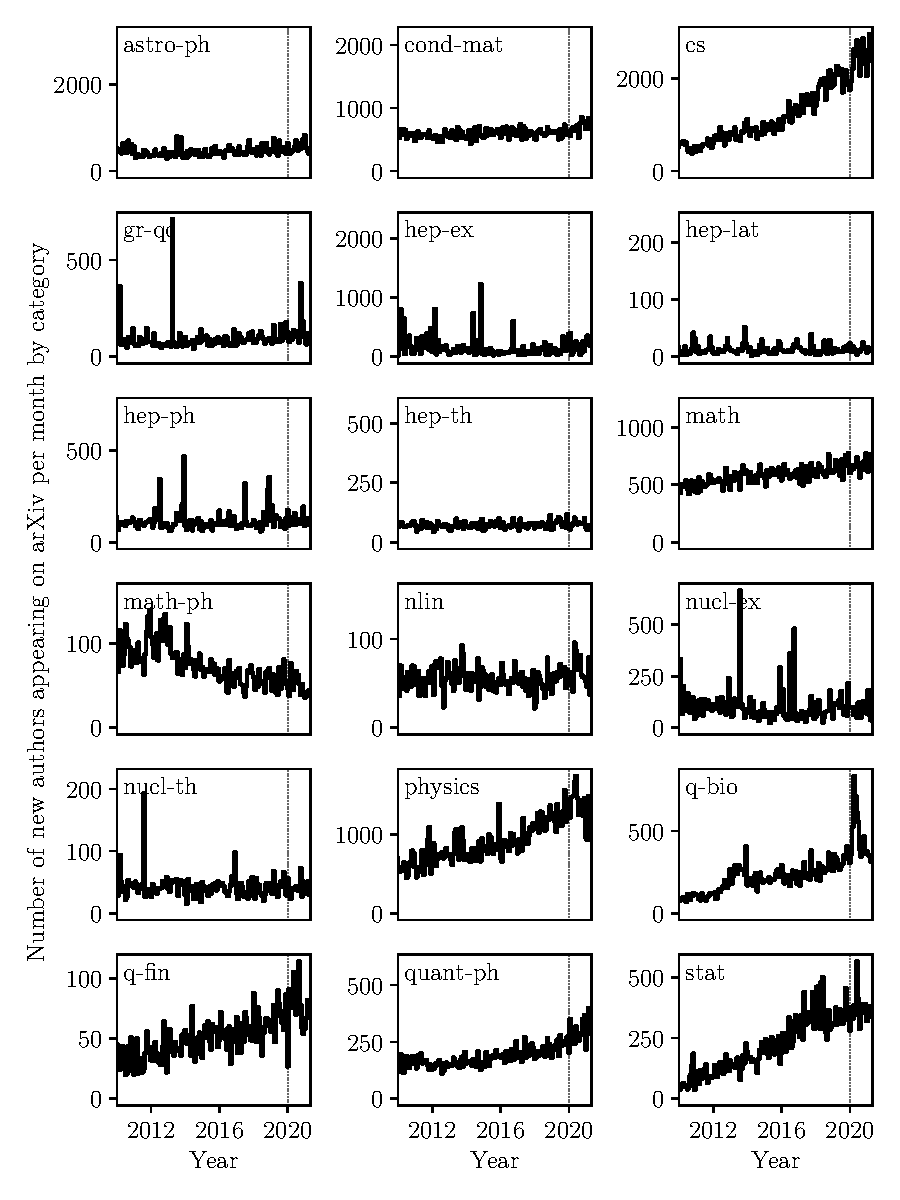
\includegraphics[width=\textwidth]{new-authors-segmented-by-field}
	\caption{The number of new author names appearing in the literature by field. Fields established well before 2007 (e.g., astro-ph) show an apparent influx of authors at the time the data starts (2007). These author names are dominated by established academics. The slow change in new author count after 2010 approximates the net number of new academics joining the field. Note the spike in new authors in quantitative biology in 2020.}
		\label{fig:new-authors-segmented-by-field}
\end{figure}

 
  \begin{figure}
     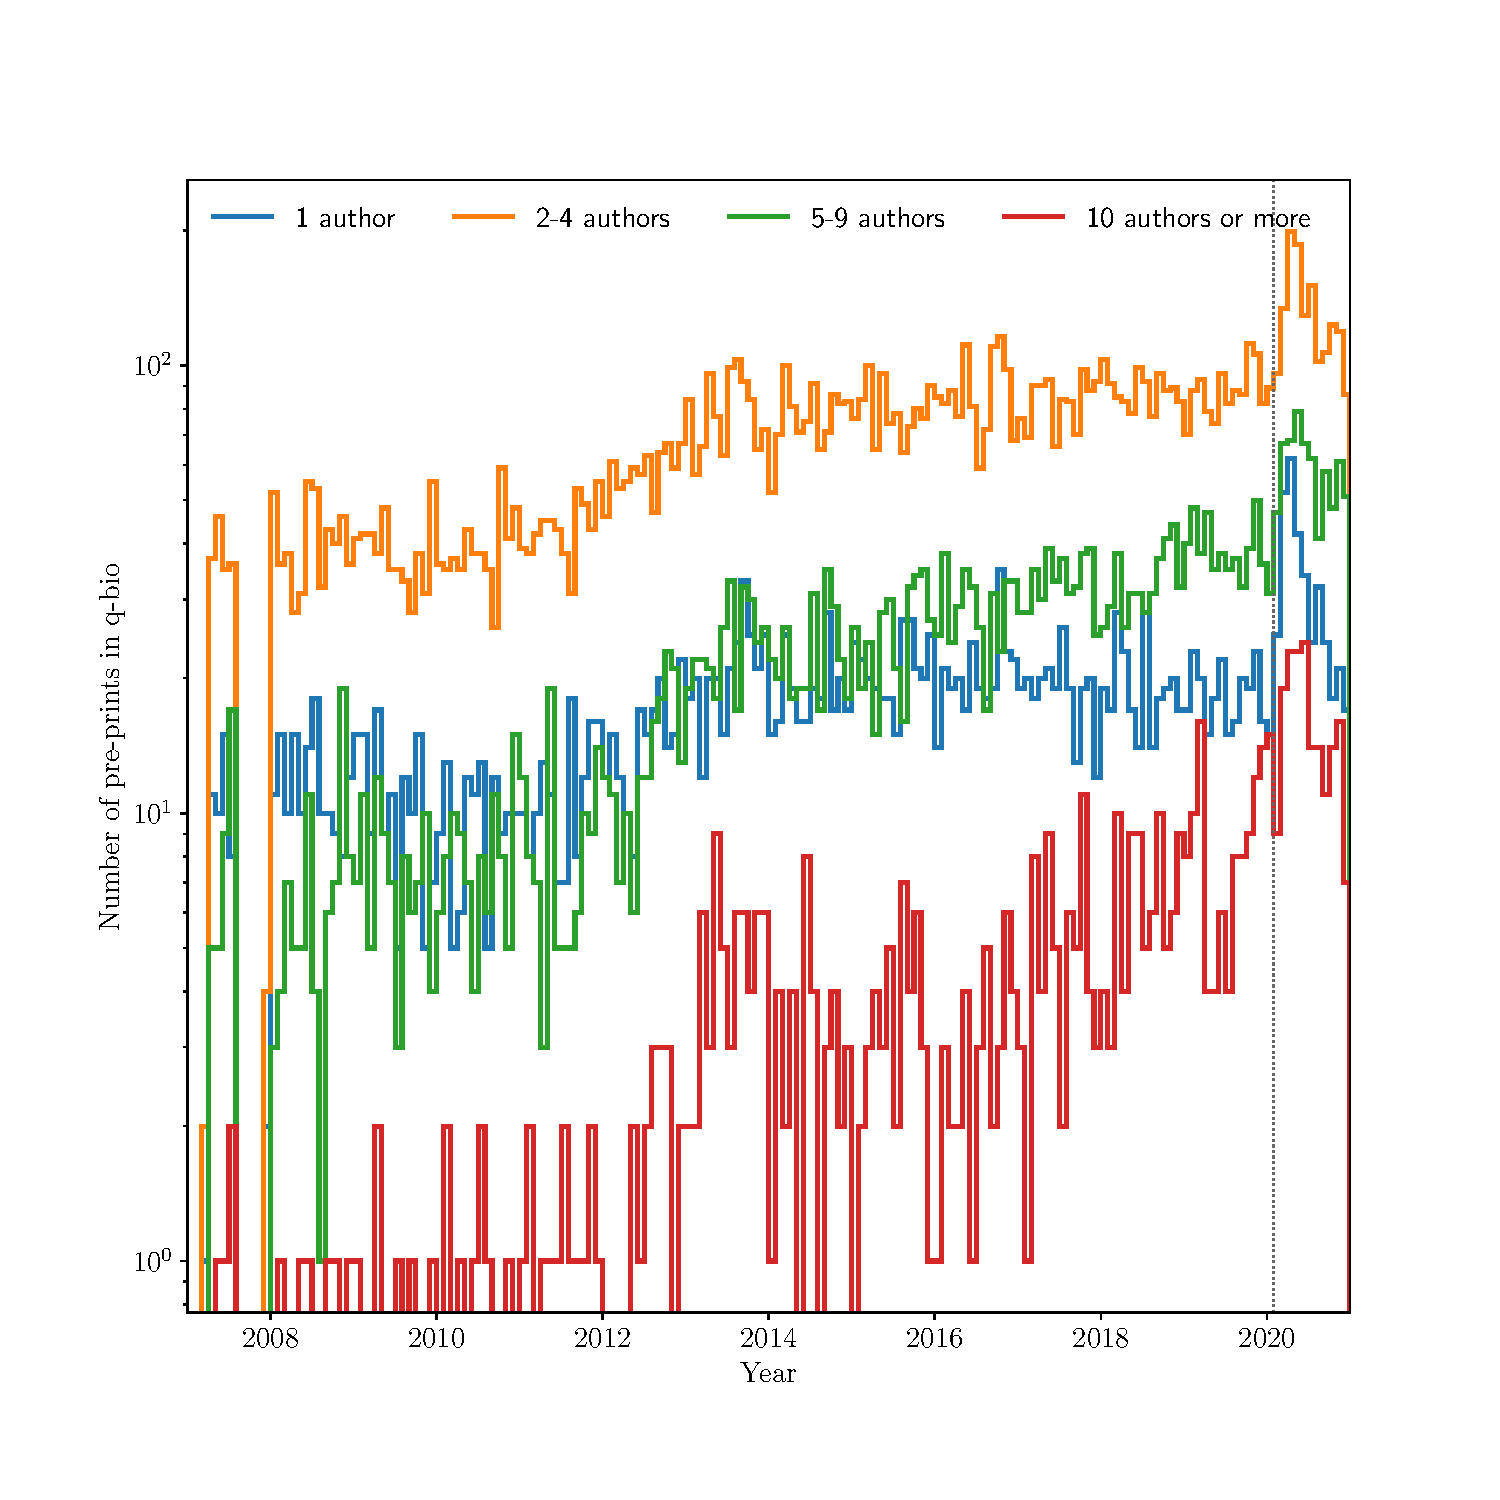
\includegraphics[width=\textwidth]{q-bio-pre-prints-segmented-by-author-count}
     \caption{The increase in quantitative biology pre-prints in 2020 cannot be attributed to large collaborations. Here we segment q-bio pre-prints by the number of authors, showing that in 2020 a sharp increase was observed for single-author papers and small (2-4 authors) collaborations.}
     \label{fig:q-bio-pre-prints-segmented-by-author-count}
  \end{figure}

\begin{figure}
	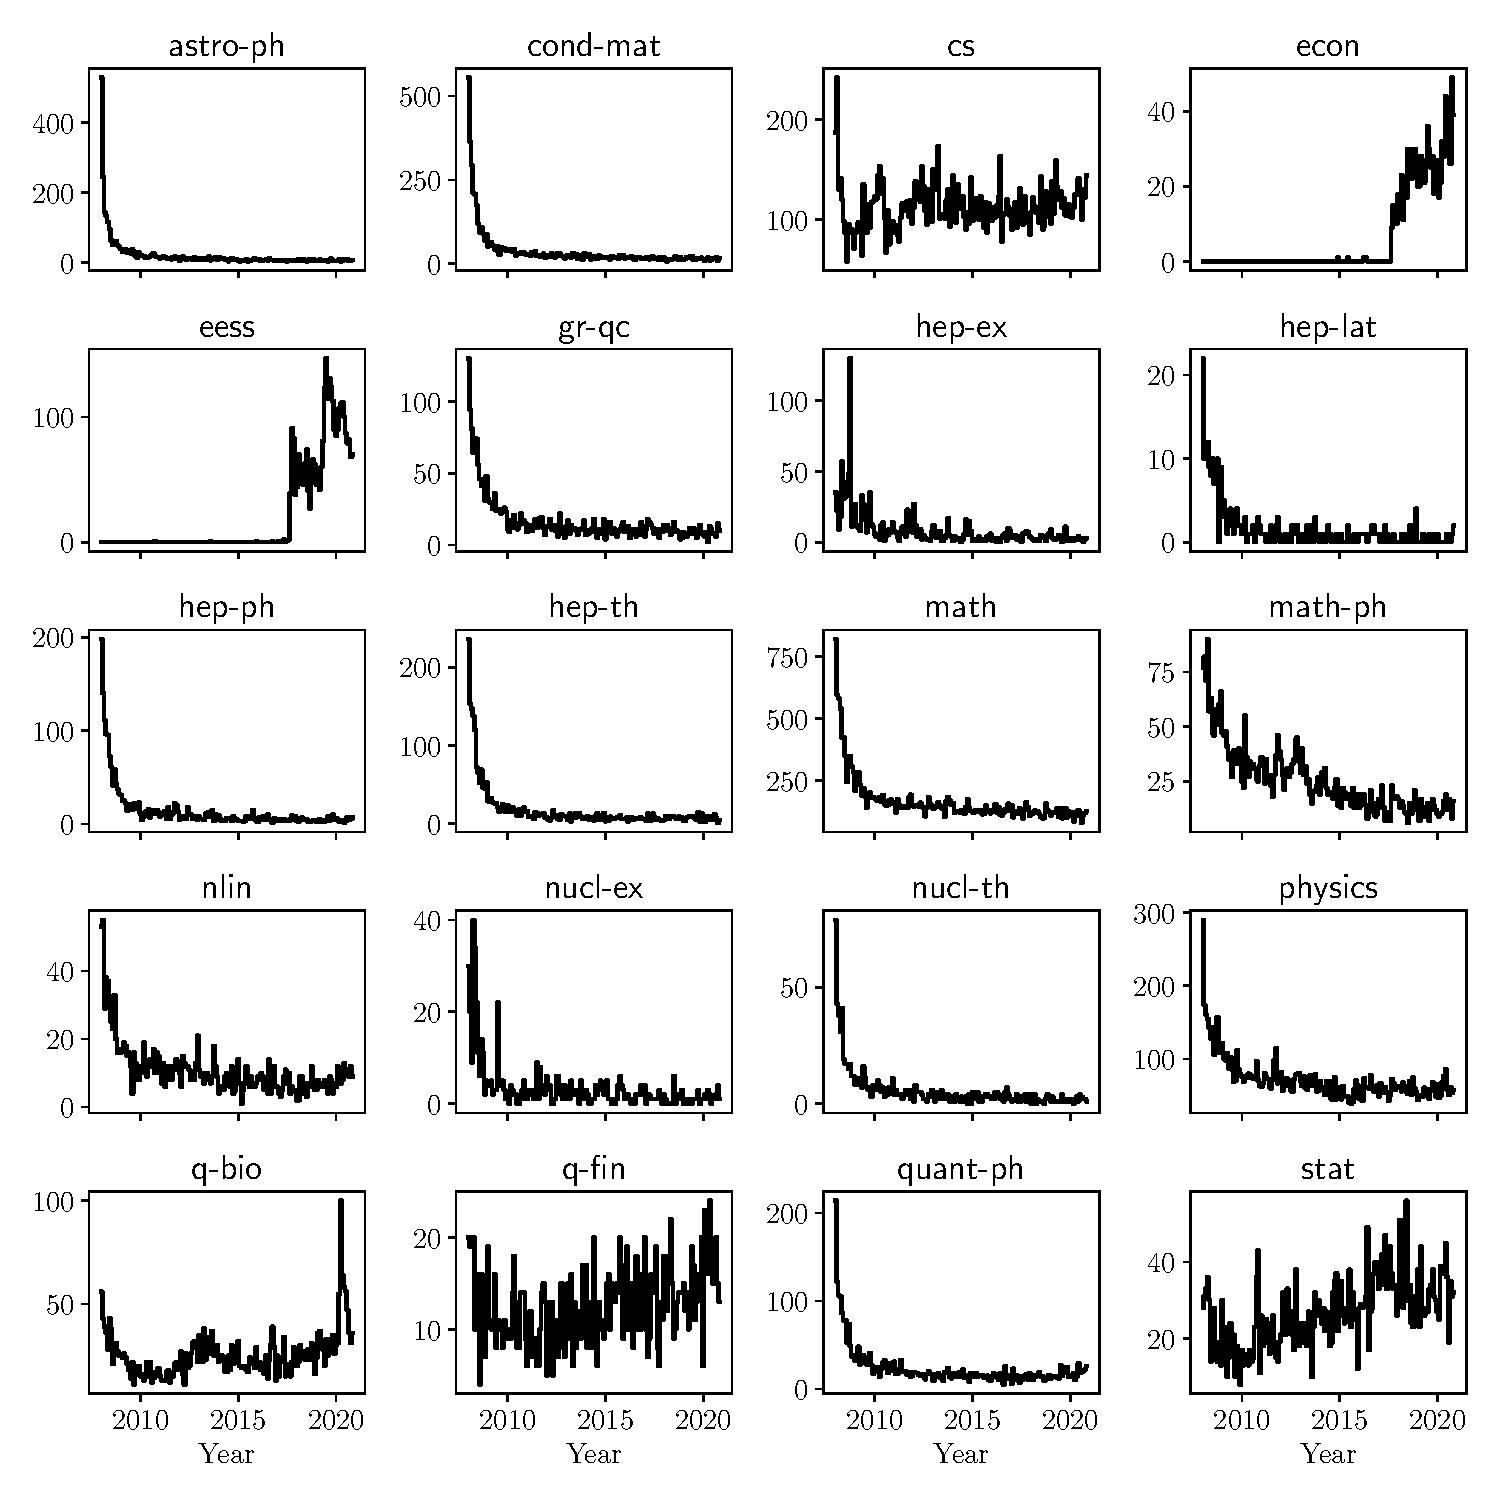
\includegraphics[width=\textwidth]{pre-prints-with-entirely-new-authors}
	\caption{The number of pre-prints appearing per field where all authors have never appeared in the literature for that field before. A sharp increase remains present for quantitative biology (q-bio), representing an influx of pre-prints entirely written by authors who had never posted to \arxiv/q-bio before.}
		\label{fig:pre-prints-with-entirely-new-authors}
\end{figure}


  \begin{figure}
     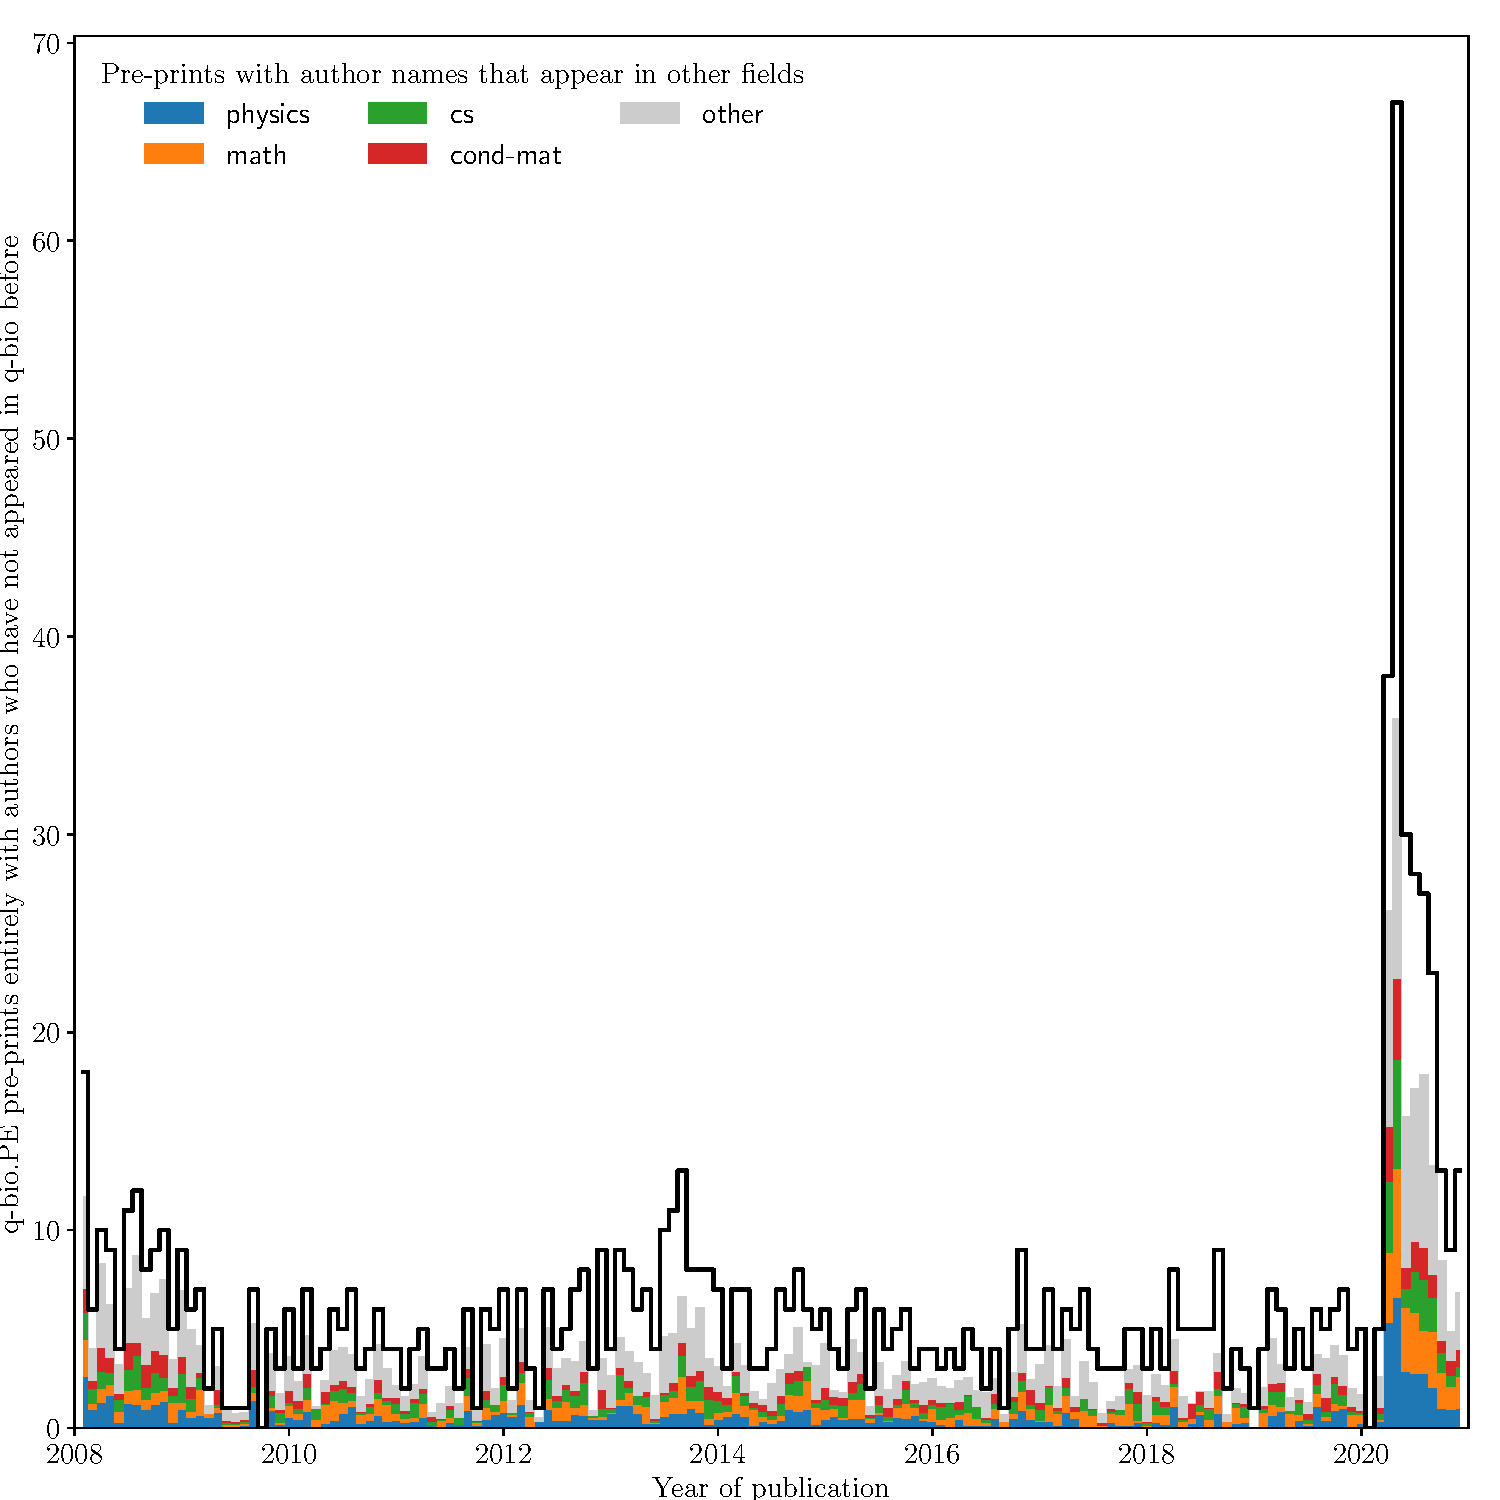
\includegraphics[width=\textwidth]{q-bio-pre-prints-with-author-overlap}
     \caption{Many physicists and mathematicians posted pre-prints to quantitative biology in 2020 for the first time. Pre-prints in \emph{Populations and Evolution} (q-bio.PE) that are written entirely by authors who have never before appeared in quantitative biology (q-bio). The area shows the number of pre-prints where those authors have appeared in other fields.
     }
   	\label{fig:q-bio-pre-prints-with-author-overlap}
	\end{figure}	



% \begin{figure}
%     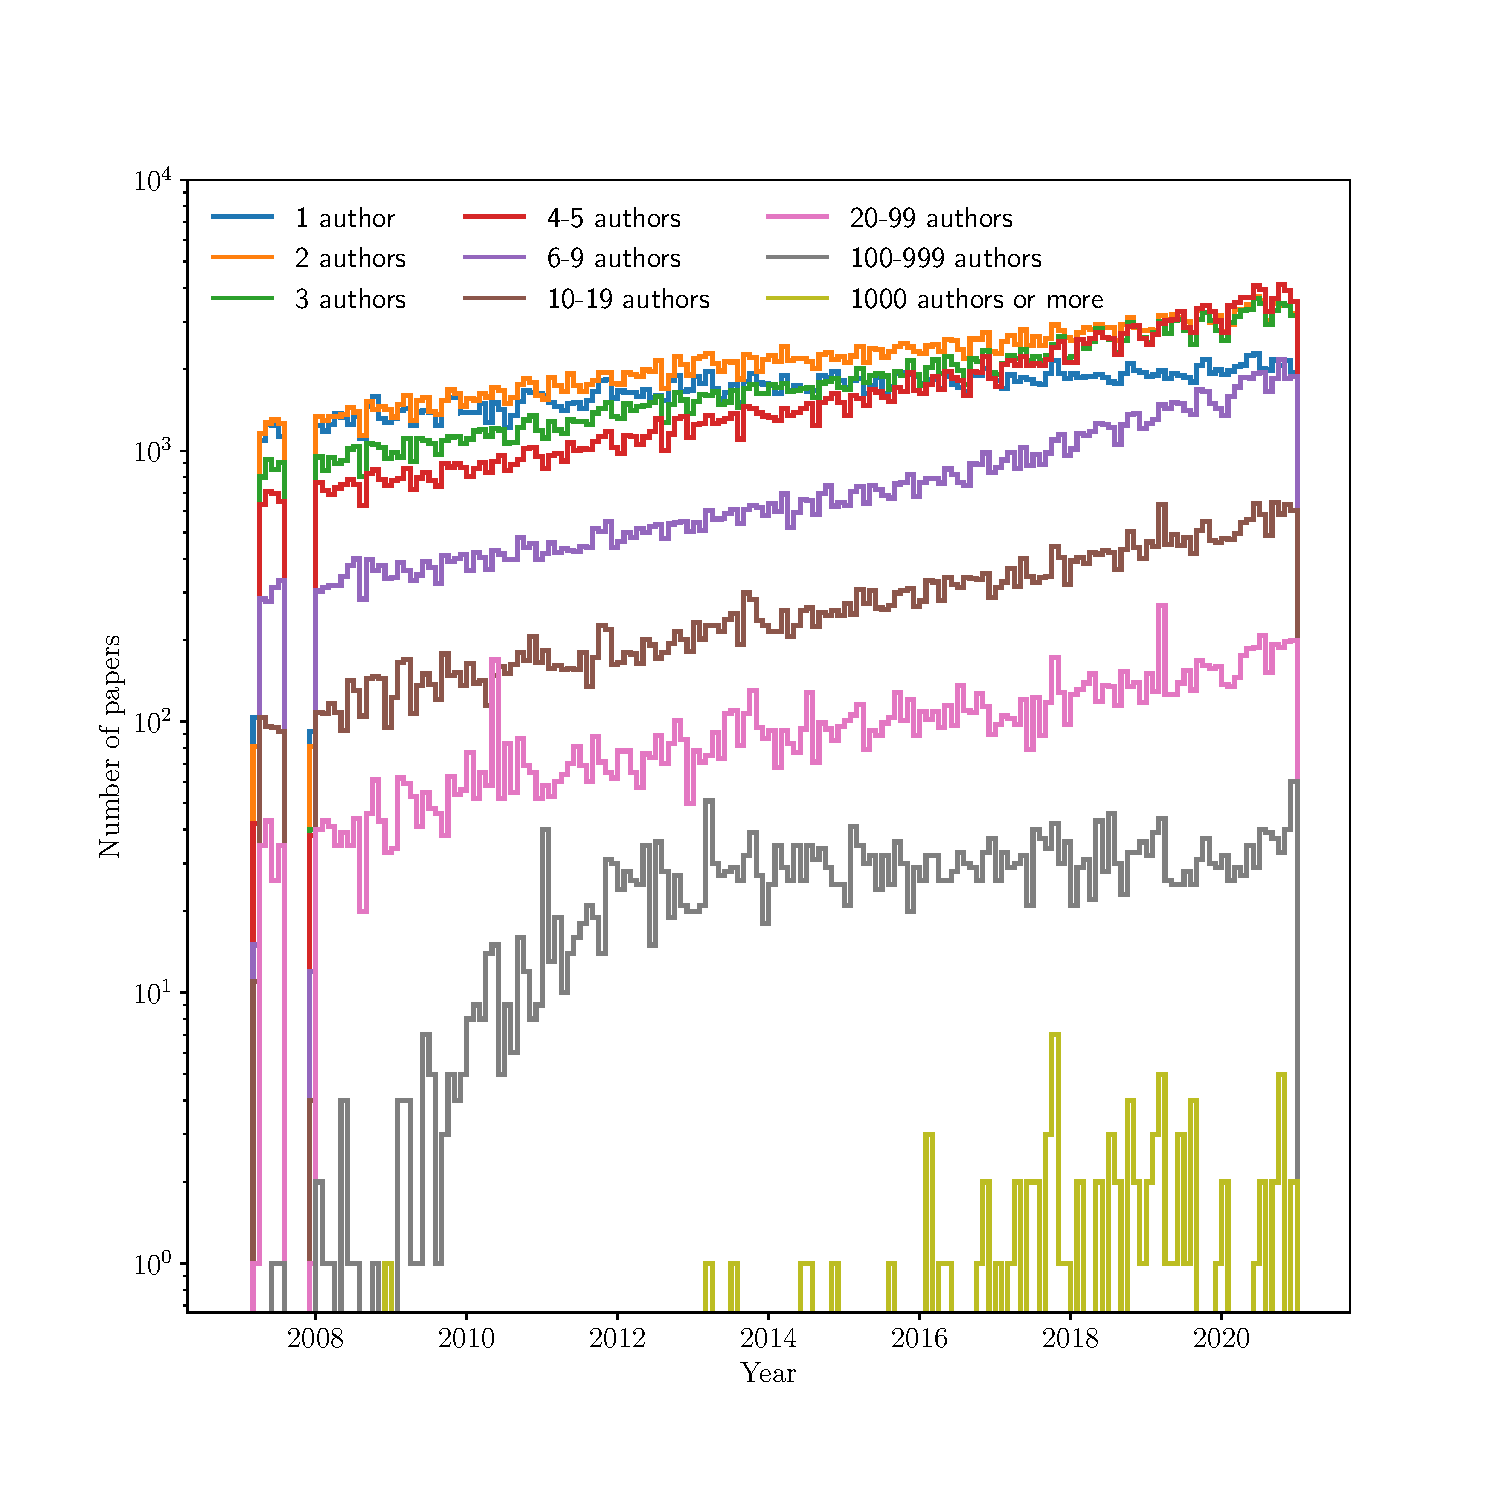
\includegraphics[width=\textwidth]{pre-prints-segmented-by-author-count}
%     \caption{Each year academics are writing more papers, with more co-authors. The typical size of the largest collaboration papers continues to increase. Single author papers are becoming rarer with time.}
%     \label{fig:pre-prints-segmented-by-author-count}
% \end{figure}


% \begin{figure}
%     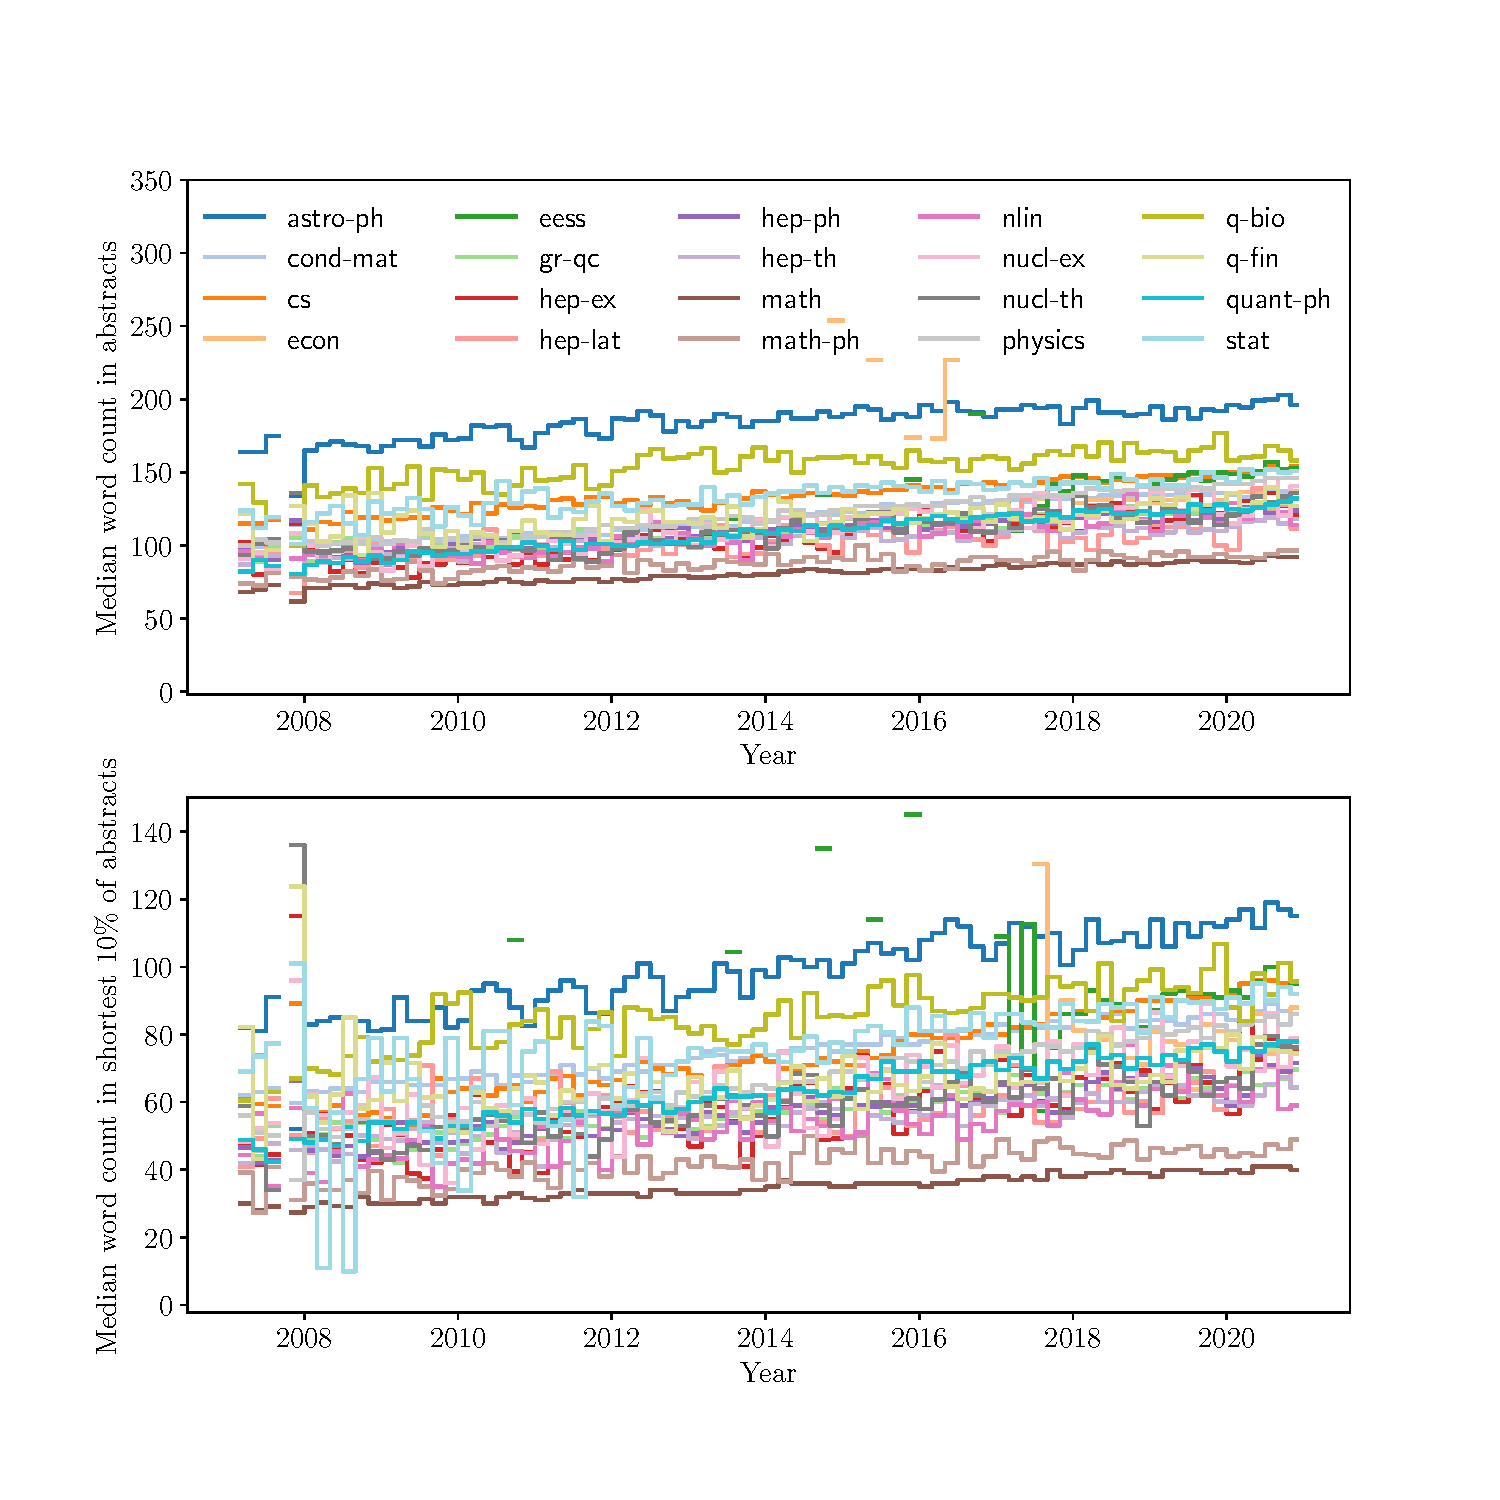
\includegraphics[width=\textwidth]{pre-prints-abstract-length}
%     \caption{The typical length of pre-print abstracts indicates that academics are writing longer papers (top). Even the shortest 10\% of abstracts in a given time bin are increasing in length (bottom).}
%     \label{fig:pre-prints-abstract-length}
% \end{figure}
 

%\begin{figure}
%	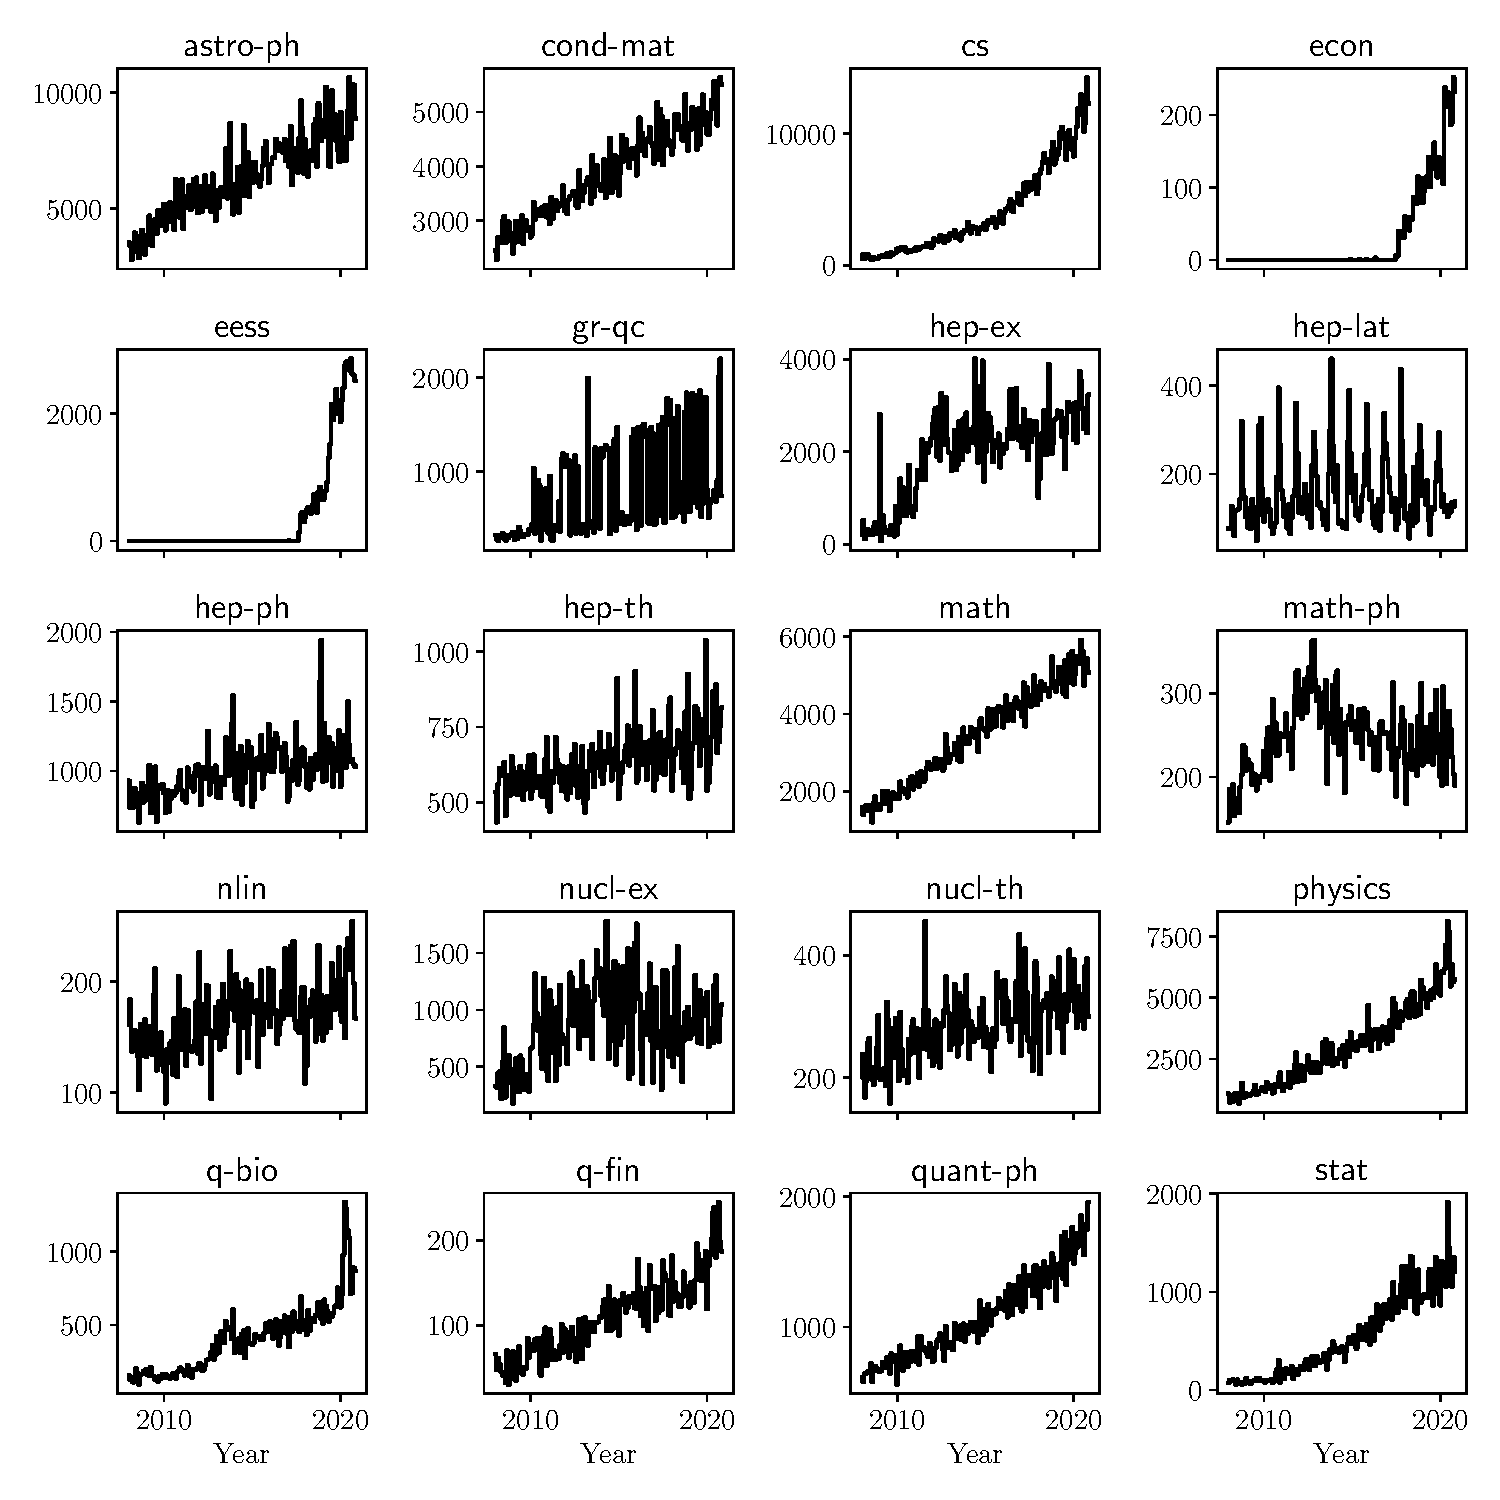
\includegraphics[width=\textwidth]{unique-authors-segmented-by-field}
%	\caption{The number of unique author names in each field as a function of time.}
%		\label{fig:unique-authors-segmented-by-field}
%\end{figure}
 




\begin{figure}
	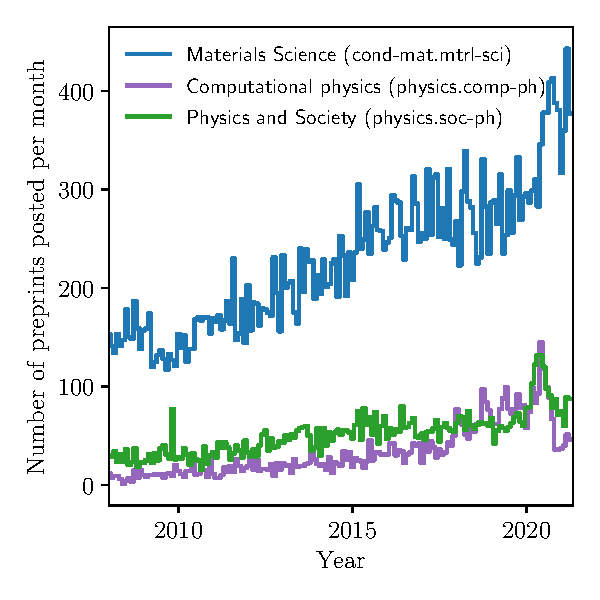
\includegraphics[width=\textwidth]{winners-and-losers-of-covid}
	\caption{The number of pre-prints in selected sub-fields where the pandemic may have caused a change in publication rates.}
		\label{fig:winners-and-losers-of-covid}
\end{figure}







\section*{References}

\begin{thebibliography}{30}
%\bibitem{Iben_1967} Iben, I., Jr. Stellar Evolution. VI. Evolution from the Main Sequence to the Red-Giant Branch for Stars of Mass 1 $M_{sun}$, 1.25 $M_{sun}$, and 1.5 $M_{sun}$. \emph{Astrophys. J.} \textbf{147}, 624, doi:10.1086/149040 (1967).
\end{thebibliography}

\bibliographystyle{naturemag}


\begin{addendum}
\item[Supplementary Information] ~\\Supplementary information is linked to the online version of the paper at www.nature.com/nature.
\item[Acknowledgements] Peter Skands (Monash University) 
						and Ross Young (University of Adelaide) for comments on publication trends.

 \item[Author Information] Reprints and permissions information is
   available at www.nature.com/reprints. The authors declare that they
   have no competing financial interests. Correspondence and requests
   for materials should be addressed to andrew.casey@monash.edu
\end{addendum}

\begin{methods}

\section*{Data retrieval}

The \arxiv\ supports an Open Archive Initiative [REF] protocol to access metadata for individual pre-prints, given an identifier. A pre-print's identifier is defined by the year and month that the pre-print was posted, and the number of pre-prints already posted in that month (across all fields). We first retrieved the total number of pre-prints posted to the \arxiv\ each month [REF], and used this to generate all possible identifiers. For each identifier we retrieved the title, author name(s), abstract, research field(s), and the date the pre-print was first posted. For pre-prints posted to \arxiv\ prior to 2007, the primary research category is needed to generate the \arxiv\ identifier. Since the primary research category is not readily available for all pre-prints \emph{a priori}, we chose to exclude pre-prints posted earlier than 2007. This data set includes metadata for 1,379,332 pre-prints posted between 2007-03-30 and 2020-12-30, inclusive.


\section*{Long-term modelling of pre-print counts}

\todo{Model the long-term paper counts with a Poisson process.}


\section*{Uniquely identifying authors}

The metadata available to us does not include institutional affiliations, or identifiers that would uniquely identify an author. For these reasons, we have taken steps to minimise the effects of name confusion. There are two primary ways that name confusion could impact our inferences. In the first scenario, two people with the same name are amalgamated and treated as a single author that is on average twice as productive (or more, for very common names) as other authors. In the second scenario, an author will sometimes publish as `A.~B.~Smith', and other times publish as `A.~Smith'. A careful exploration of the data shows that this is a very frequent scenario, and if left uncorrected, would appear as many `unique' authors with half as many publications on average.

We have taken a simple approach to address name confusion. We first define a unique author by family name and the initial of the first given name (`Family-name, I.'), such that we intentionally group together authors that may share the same initial of their second given name. While our approach to name confusion is grossly simple, it is unlikely that these choices have any substantial impact on our inferences. Any common name is likely to appear in the literature early in the data set, and will not impact the conclusions we draw about how publishing changed in 2020. While common names will appear between different fields (e.g., quantitative biology and physics), by showing this as a function of time we get an intrinsic measure of the name ambiguity between fields, and we see the increase in overlap when a spike in quantitative biology papers occurs. 
Nevertheless, we manually inspected \todo{hundreds} of quantitative biology pre-prints that entirely consisted of `new authors' and cross-referenced these with Google Scholar to confirm that these authors were established researchers in other fields, and not biologists posting pre-prints for the first time.

\section*{Segmenting by research field}

Pre-prints posted to the \arxiv\ can be cross-listed in multiple fields of research, and multiple sub-fields. For example, one pre-print may have a primary field of research as stellar astrophysics (astro-ph.SA) and be cross-listed in computer science. The corresponding author must always specify the primary and additional fields of research. Throughout this work when we segment by primary research field, we take the primary parent research field provided (in this example, astro-ph). We ignore the cross-listings, as these are not always provided for pre-prints, and not always appropriate for appropriating research productivity between different fields. When we segment pre-prints by sub-field, we similarly take the primary sub-field provided and ignore any cross-listings.

\section*{Code availability}
The software developed to retrieve and analyse these data is publicly accessible online\footnote{https://github.com/andycasey/arxiv-covid}. All data was sourced from the \arxiv.

\end{methods}


%\section*{Additional References}
%\begin{thebibliography}{1}
%\bibitem[31]{LAMOST} Luo, A.-L. \emph{et al}. The First Data Release (DR1) of the LAMOST general survey. \emph{Res. Astron. Astrophys.} \textbf{15}, 1095, doi:10.1088/1674-4527/15/8/002 (2015).
%\end{thebibliography}

\bibliographystyle{naturemag}


\end{document}



